\documentclass[preprint]{sigplanconf}

% The following \documentclass options may be useful:
%
% 10pt          To set in 10-point type instead of 9-point.
% 11pt          To set in 11-point type instead of 9-point.
% authoryear    To obtain author/year citation style instead of numeric.

%% To compile under Ubuntu:
%% cd Calico/papers/dsl-13/
%% sudo apt-get install texlive-latex-base
%% sudo apt-get install texlive-fonts-recommended
%% make

\usepackage{amsmath}
\usepackage{graphicx}
\usepackage{color}
\usepackage{listings}

\begin{document}

\definecolor{mygreen}{rgb}{0,0.6,0}

\lstset{showspaces=false, basicstyle=\footnotesize, showstringspaces=false, 
        captionpos=b, frame=single, numbers=left, commentstyle=\color{mygreen}}

\conferenceinfo{SPLASH DLS'13}{October 28, 2013, Indianapolis, Indiana, USA.} 
\copyrightyear{2013} 
\copyrightdata{ACM} 

\titlebanner{Submitted to SPLASH DLS'13}        % These are ignored unless
%%\preprintfooter{short description of paper}   % 'preprint' option specified.

\title{Calico: An Ecosystem for Dynamic Languages}
%% \subtitle{Subtitle Text, if any}

\authorinfo{Douglas S. Blank}
           {Bryn Mawr College\\Department of Computer Science\\Bryn Mawr, PA 19010 USA}
           {dblank@cs.brynmawr.edu}

\authorinfo{Mark F. Russo, Ph.D.}
           {Rowan University\\Department of Computer Science\\Glassboro, NJ 08028 USA}
           {russomf@gmail.com}

\authorinfo{James B. Marshall}
           {Sarah Lawrence College\\Department of Computer Science\\Bronxville, NY 10708 USA}
           {jmarshall@slc.edu}

\maketitle

\begin{abstract}

\end{abstract}

The Calico project was designed to be a dynamic languages ecosystem
for learning, exploring, creating, and using dynamic languages, both
individually, and in cooperation with each other. It defines a
multi-language, multi-context programming framework and learning
environment for computing education and research. The ecosystem is
designed to support several interoperable programming languages
(including Python, Scheme, and a drag-and-drop languages, called
Jigsaw) running on a universal virtual computer.  We plan that that
Calico will provide a long-term, robust ecosystem that can be used to
create and sustain a community of researchers, educators, and students
working together in dynamic languages research.

\category{D.3.4}{Programming Languages}{interpreters, runtime environments}

\terms
Languages, Experimentation

\keywords 
Integrated Development Environment, dynamic languages,
virtual machine, language implementation, language interoperations

\section{Overview}

The Calico Project defines a collection of technologies designed to
create an ecosystem for dynamic languages. The Calico ecosystem has a
number of interesting properties: 1) allows multiple dynamic languages
to interact and interoperate; 2) libraries written for the ecosystem
are usable by all of the languages as if they were native to each
language; 3) provides a smooth continuum of experience for the
beginning computer programmer; 4) exposes a unified interface for
exploring a variety of dynamic languages; and 5) is an open-source
testbed for developing new concepts in dynamic languages. As such,
Calico defines a useful ecosystem for students, educators, and
developers wishing to explore computer science and pedagogy.

Calico is defined by three layers of technologies: a universal virtual
computer, a dynamic language runtime, and support libraries and
executables. In addition, an Integrated Development Environment (IDE)
pulls all of these pieces together, for use by students and researchers. As
implemented, Calico languages can all live and operate in the same
space, share variables and code, and the code can run competitively
fast. The following sections go into the details of each of the pieces
that comprise the Calico ecosystem.

\subsection{Universal Virtual Computer}

From the programmer's perspective, the foundation of Calico is a
``universal virtual computer''. The dynamic language programmer should
be able to write code capable of modern functionality without having
to worry about the details of the operating system or underlying
hardware. For example, the programmer should be able to write programs
capable of: turning text to speech; playing audio files; defining
functions that can be used for tone generation; creating graphical
user interfaces with unconstrained drawing abilities; reading and
writing standard image formats; and providing access to modern
input/output hardware devices, such as gamepads, joysticks, webcams,
and robots. In addition, such a system should be easy to install and
maintain, with limited need for platform-specific
dependencies. Finally, we believe that a long term platform for
research and education should be free, both in terms of price and
ability to distribute and alter. Thus, the programmer should be able
to program to a complete, easily-accessible, free, modern, universal
virtual computer. This section examine the components of a universal
virtual computer.

\subsubsection{Virtual Machine}

A large portion of the universal virtual computer is defined by a
``process virtual machine.'' There are a number of process virtual
machines (VMs) one could use for a dynamic language ecosystem. We
wanted a VM with a large and active development community, and so
excluded more narrowly-focused VMs such as the Squeak Virtual Machine
\cite{squeakvm}. Oracle's Java and Microsoft's .NET are two VMs that
both define viable possibilities: both have object-oriented
programming languages, compilers, and associated virtual machines and
runtimes. The Java VM (JVM) has the Java language (among other
possibilities), and .NET has the C\# language (among other
possibilities). Both systems compile to bytecode that is executed by
their respective virtual machines' runtime.

Although both VMs have served as the foundation for dynamic languages,
Java does not have a complete and robust open-source
implementation. On the other hand, .NET’s virtual machine components,
called the Common Language Infrastructure (CLI), have been clearly
defined in a pair of Ecma standards, specifically Ecma \#334 and Ecma
\#335 \cite{ecma-standards}, and is protected by a promise from
Microsoft not to sue \cite{microsoft-community-promise}. More
importantly, these standards have been implemented independently by
Mono as open source. We have put a high value on having a complete,
independent, and open source ``stack'' of robust software
layers. Although one could debate which system is more ``open'', we
decided to select the CLI as implemented by Mono \cite{mono}. we will
refer to Mono's implementation of the CLI as MVM (for Mono Virtual
Machine).

However, we are not limited to only MVM-based technologies. Using IKVM
(described below) we are able to utilize code compiled for the Java
VM. In this manner, we have assembled components that bring together
the best of both of these two virtual machine systems. In effect, we
have a ``universal virtual machine'' that can use a wide variety of
available open-source libraries on a varied set of operating
systems. One such library is the Dynamic Language Runtime described in
the next section.

\subsubsection{Dynamic Language Runtime}

Although the MVM and the JVM both define everything necessary to
implement a dynamic language, neither has built-in support for
allowing such dynamic languages to interoperate. That is, even though
a variety of languages can be compiled to either VM, there is little
common infrastructure in the VM itself. Without a dynamic language
infrastructure, it is difficult for languages defined in the VM to
define dynamic objects, and to share environments, data structures,
objects, or functions. Two Java Specification Requests have been made
to add such functionality to Java: JSR-223 would add language hosting
and JSR-292 would add dynamic binding \cite{wu-2010}. In fact, there are a
number of projects underway to make the JVM more flexible for use with
dynamic languages, including: the Da Vinci Machine \cite{java-davinci}
as the reference implementation of JSR-292; Project Lambda
\cite{java-lambda} adds lambda to the JVM; Project Jigsaw adds
supported for importing versioned modules \cite{java-jigsaw}; and
Nashorn \cite{java-nashorn} adds caches for dynamic invokes. When
complete, these technologies will extend the Java technologies to make
them much more suitable for dynamic languages.

On the other hand, the MVM has an existing, mature framework for
implementing languages called the Dynamic Language Runtime (DLR)
\cite{dlr-microsoft}, and at least three dynamic languages have been
written using the DLR: IronPython \cite{ironpython}, IronRuby
\cite{ironruby}, and PowerShell \cite{powershell}. The DLR contains
many tools and technologies for language writers to create languages,
and abilities for the languages to interoperate. Calico includes the
DLR, and contains versions of IronPython and IronRuby. A language need
not use the functionality of the DLR to be used in Calico, but this
functionality is required for a language to be considered
\textit{first-class} (described below).

The DLR provides the following \cite{dlr-wikipedia}:
\begin{itemize}
\item A dynamic, shared type system 
\item Dynamic method dispatch
\item Dynamic code generation
\item Hosting API
\end{itemize}

A new object type, DynamicObject, was created to implement this
functionality. DynamicObject was initially defined in the DLR as an
external library, but now has been incoprorated into .NET 4.5, the C\#
language, and Mono. DynamicObject is a base class for creating objects
that determine the behavior dynamically at runtime. The DLR contains
all the support necessary for creating, parsing, and executing modern
dynamic languages. However, even with the DLR and the virtual machine,
there are still a large set of functions that a modern programmer
would expect from a universal computer (including audio and
graphics). We now explore these supporting libraries.

%%  DLR: DynamicObject, cache point, AST, hosting, environment]

\subsection{Supporting Libraries}

To create a universal virtual computer, we need to have a set of
capabilities on top of the virtual machine and dynamic language
runtime that run the gamut from audio to graphics. Of course,
operating systems and hardware vary wildly. Fortunately, there are
open source libraries for the MVM that cover these requirements. For
graphics, we selected Gtk\# \cite{gtk-sharp} which wraps low-level
C-based libraries. For accessing audio and hardware devices (such as
gamepads), we selected the Simple DirectMedia Layer (SDL)
\cite{sdl}. SDL is quite popular in open source, providing additional
capabilities for many projects, including pygame
\cite{pygame}. Finally, we also added espeak \cite{espeak} to provide
cross-platform text-to-speech functionality.

%% [FIXME: Gtk. SDL. espeak. graphviz. ]

The MVM and the above mentioned libraries form the lowest level of the
virtual computer. These libraries are machine-dependent, and, as such,
must be compiled for each platform. We attempted to create the fewest
number of machine-specific dependencies to make the virtual computer
easy to maintain and port to new architectures.  Finally, after this
low-level set of dependencies are satisfied, additional libraries can
be written in a machine-independent fashion using the MVM, or written
with the JVM and converted with IKVM to the MVM.

IKVM is an interesting open source project that translates binary code
between MVM/.NET and the JVM \cite{ikvm}. It has the ability to make
code compiled for the JVM availble to the MVM, and, likewise, to make
code compiled for the MVM (or .NET in general) available to the
JVM. We see an example of IKVM with Calico Java (discussed below).

Combined with the MVM and DLR, these libraries complete the
functionality of a universal virtual computer so that one can write
programs that utilize graphics user interfaces (including widgets,
freestyle pixel manipulation, event handlers, and image formats),
audio (including text-to-speech and tone generation), access to
hardware devices, and other modern functionality. One can then write
in dynamic languages with the full scope of abilities on most of the
operating systems in use, including Windows, Linux, Mac OSX, and
FreeBSD.

\subsection{Integrated Development Environment}

From the user's perspective, an important part of using any
programming language is the user interface implemented in the
Integrated Development Environment (IDE). In fact, there are many
subtle details that go into making a useful IDE. One could re-use an
existing IDE to integrate the universal virtual computer. However, we
choose to use the virtual computer to implement a new IDE. This serves
as both a test of the system, but also makes it easy to make all of
the IDE functionality accessible to the programmer. 

\begin{figure}[h!]
  \centering
     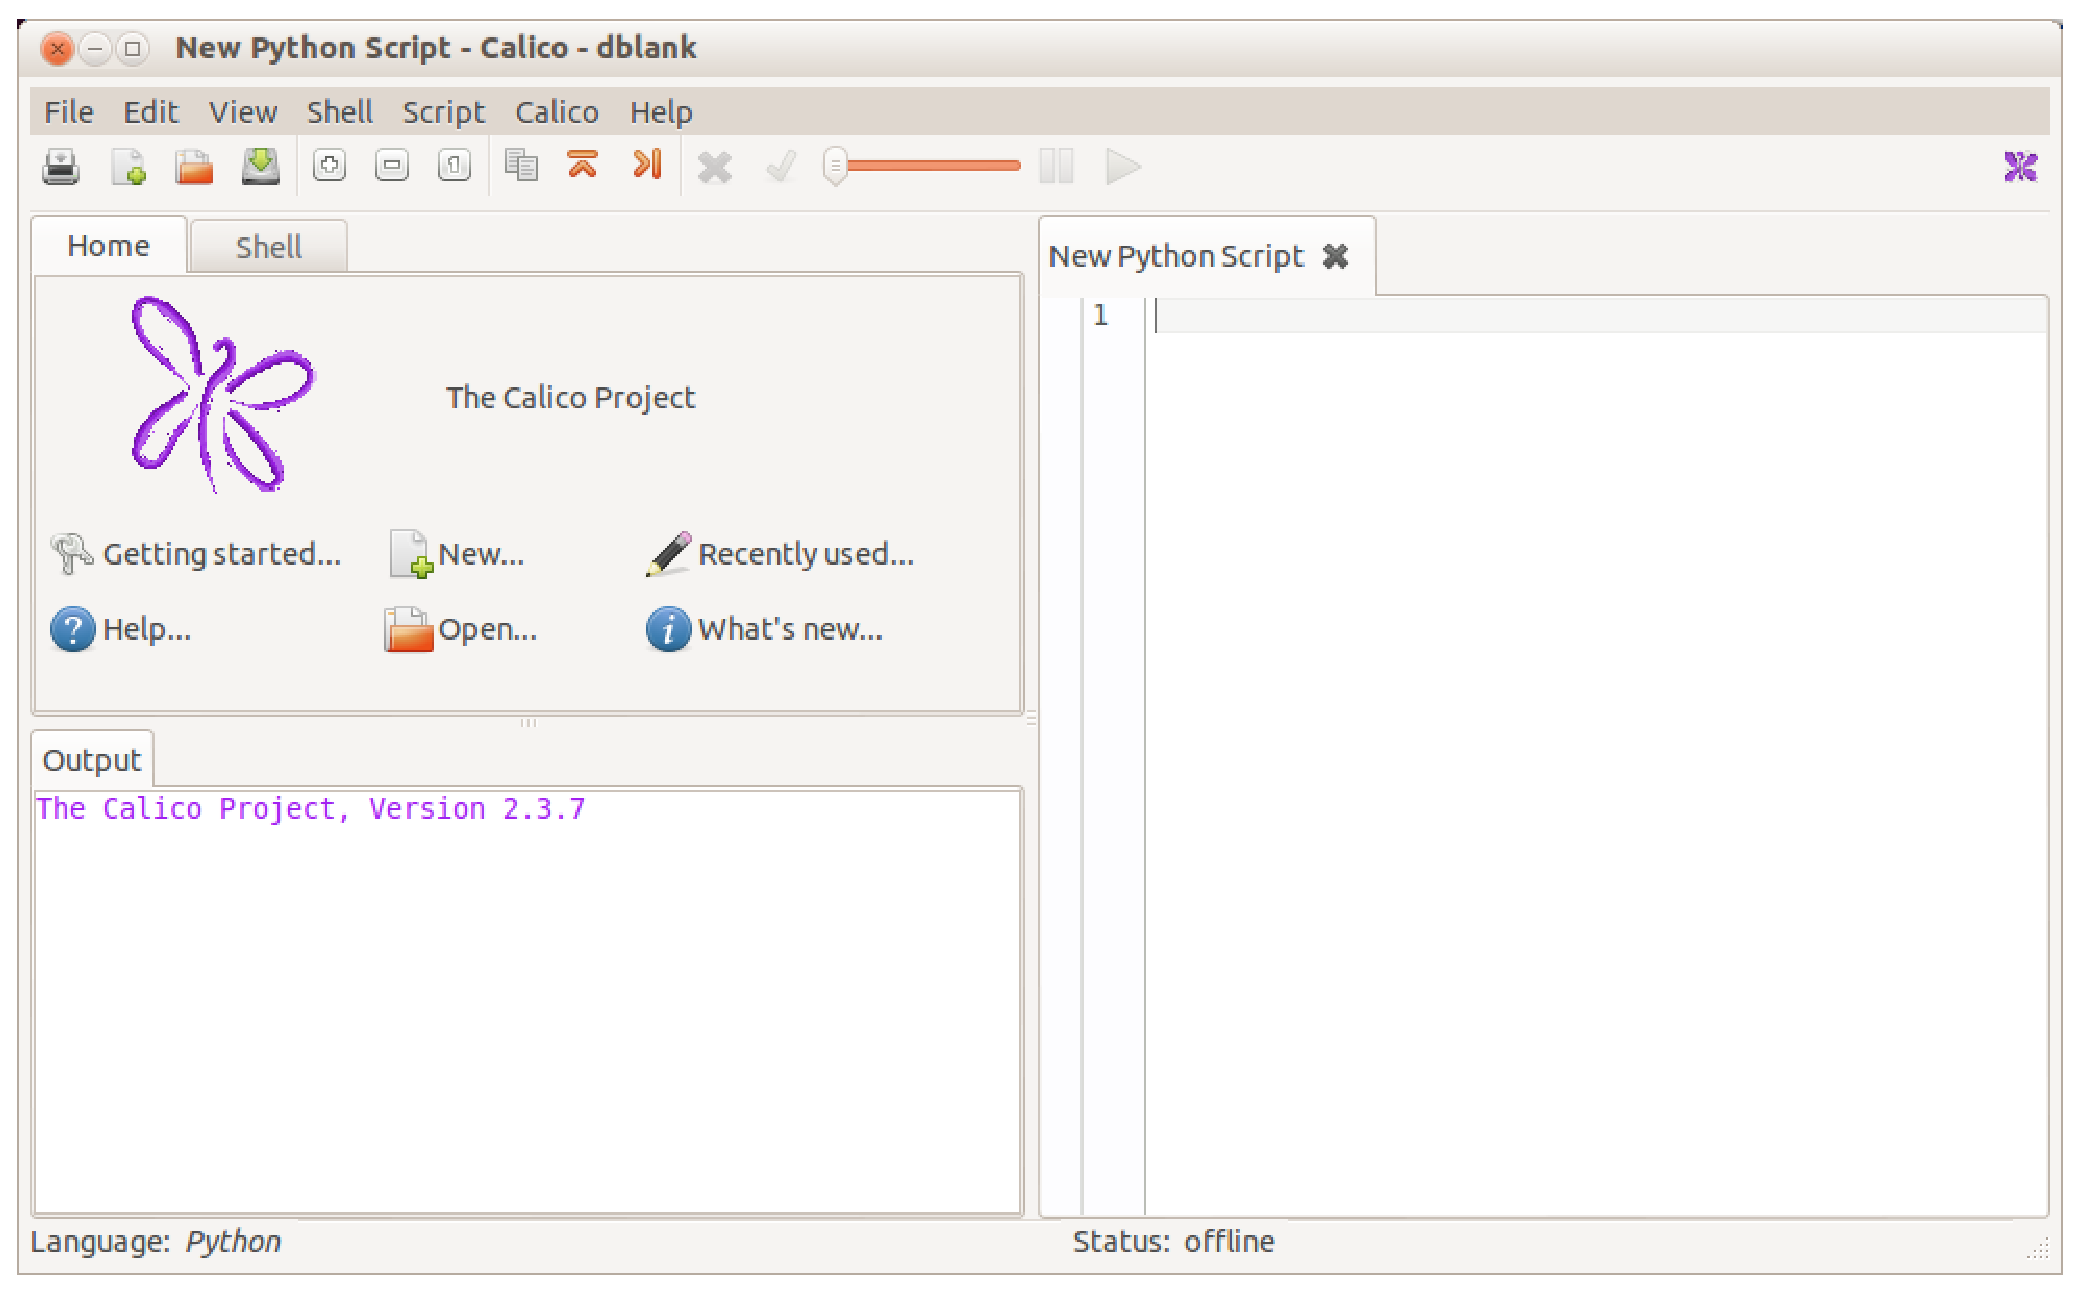
\includegraphics[width=75mm]{calico.eps}
  \caption{The Calico IDE. The IDE starts up ready to program in the
    default language. In this example, Calico Python is the default
    language.}
  \label{calico-ide}
\end{figure}

The Calico IDE, as shown in Figure~\ref{calico-ide}, is designed to be
agnostic to any particular language, or particular use. That is not to
say, however, that the IDE treats all languages identically. For
example, a visual, block-based language does not have a separate
``shell'' as interactive functionality (such as evaluate an
espression) is initiated through the visual interface. Text-based
languages need the shell for the standard read-evaluate-print loop
(REPL). Therefore, the Calico IDE rearranges slightly depending on
whether the languages is text-based or not.

\section{Languages}

A Calico language is composed of two abstract parts: a
\textit{document}, and an \textit{engine}. The document is responsible
for the visual representation and editing of scripts witten in the
language. The engine is responsible for executing the scripts. The
document and engine make up a container \textit{language} object which
also identifies whether the language is text-based, the associated
file extensions, and other language-specific details.

Not every use of Calico need be a complete language to take advantage
of the Calico infrastructure. For example, we have two ``languages''
(Spreadsheet, and Image) that only have a document, but not an
engine. This allows us to use the IDE for viewing and editing
spreadsheets and images. We could have made spreadsheets and images
just libraries (which they are as well). However, by raising them to
the level of a language, they can be opened and manipulated directly
by Calico.

Of course, the main purpose of Calico is to provide an environment for
using dynamic languages. We divide up languages into two kinds:
\textit{first-class} and \textit{second-class} languages. We define a
first-class language to support the following features:

\begin{itemize}

\item has an interactive program stepper
\item has a variable-speed tracer
\item ability to set breakpoints
\item ability to share variables with other languages
\item ability to call functions, execute/evaluate code and expressions from other languages,
\item ability to import Calico modules (e.g., libraries) as if they were native libraries

\end{itemize}

A second-class language is one that is missing one or more of these
features. This includes naive language ports (i.e., languages that do
not take advantage of the Calico ecosystem), possess minimal
interoperation with other languages, or inablity to import Calico
modules. Most of the languages incorporated lie somewhere between
first-class and second-class status. However, over time, we hope to
move more languages to the first-class set.

Having an environment like Calico is a useful system unto itself for
exploring dynamic language programming and interoperation. However, it
can also be of great utility to the beginning programmer. We are
currently exploring the use of Calico for computer science education
\cite{blank-etal-2012, blank-ohara-2013}. Our goal in focusing on
Jigsaw, Python, and the Scheme languages are for pedagogical
purposes. Our educational goal for using Calico is to create a smooth
learning experience, whereby students can transfer skills from one
language to the next. In the next sections we will breifly explore a
series of Calico languages.

\subsection{Calico Jigsaw}

Block-based programming languages have facilitated our ability to
introduce computer programming to novice programmers. Perhaps the most
notable example of this is Scratch \cite{scratch}. Building
executable programs by plugging together virtual blocks is a concept
that is much less intimidating to a beginner, especially when
compared with the precise syntactical rules demanded by many modern
programming languages. For this reason we sought to include a
block-based language as part of the Calico ecosystem. We named our
block language Calico Jigsaw.

The Jigsaw editor provides a palette of blocks that are dragged onto a
canvas using the mouse and connected to form an executable program
(Figure~\ref{jigsaw1}). Jigsaw blocks may have properties that can be assigned
values by the programmer. For example, the Jigsaw ``repeat'' block has
a Repetitions property that can be assigned a numeric value indicating
the number of times an inner stack of blocks should be executed. But
beyond the standard functionality expected in any block language,
Jigsaw has several additional features that we feel make it unique.

\begin{figure}[h!]
  \centering
     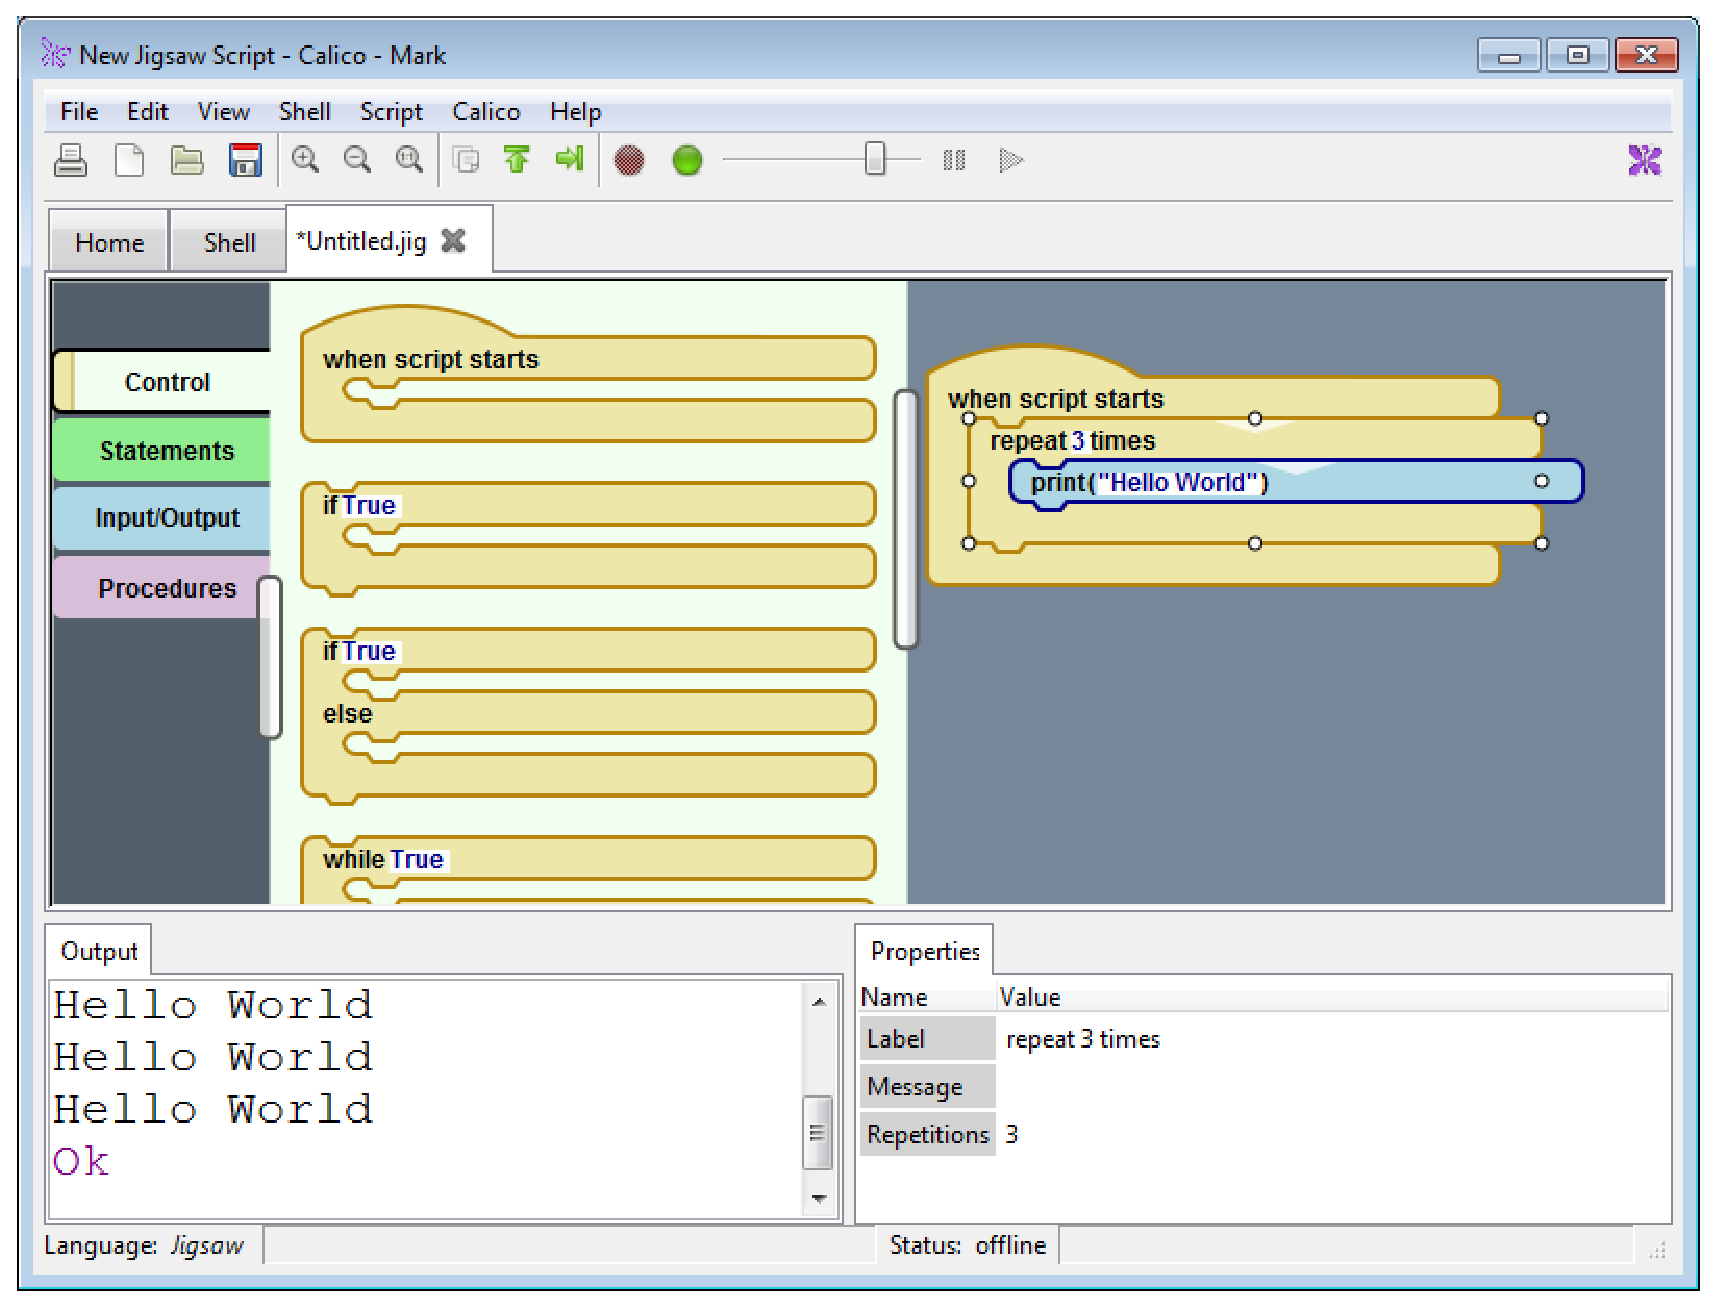
\includegraphics[width=75mm]{jigsaw1.eps}
  \caption{Jigsaw in action.}
  \label{jigsaw1}
\end{figure}

The first feature worth noting is that Jigsaw is built as a wrapper
around Python. Python thus serves as the engine for evaluating Jigsaw
expressions. We could really use any Calico language for this purpose;
however, because of our pedagogical goals, we decided to use Python as
we suggest educators use Python as the next step in a student's
computer science educational journey.

Even though Jigsaw is written in C\#, most Jigsaw statement blocks are
implemented as Python statements. This integration between C\# and
Python is possible with help from the DLR. Block statements are
compiled and held as compiled code objects that are ready to be
evaluated when the Jigsaw program runs. A consequence of this design
decision is that Python syntax often can be used directly in
Jigsaw. For example, instead of entering primitive values for block
properties, Python expressions can be substituted directly. The IfTest
conditional statement in a Jigsaw ``if'' block can be a boolean
expression written using Python syntax (Figure~\ref{jigsaw2}). We
believe that this approach better prepares the student for a smooth
transition to higher level languages.

\begin{figure}[h!]
  \centering
    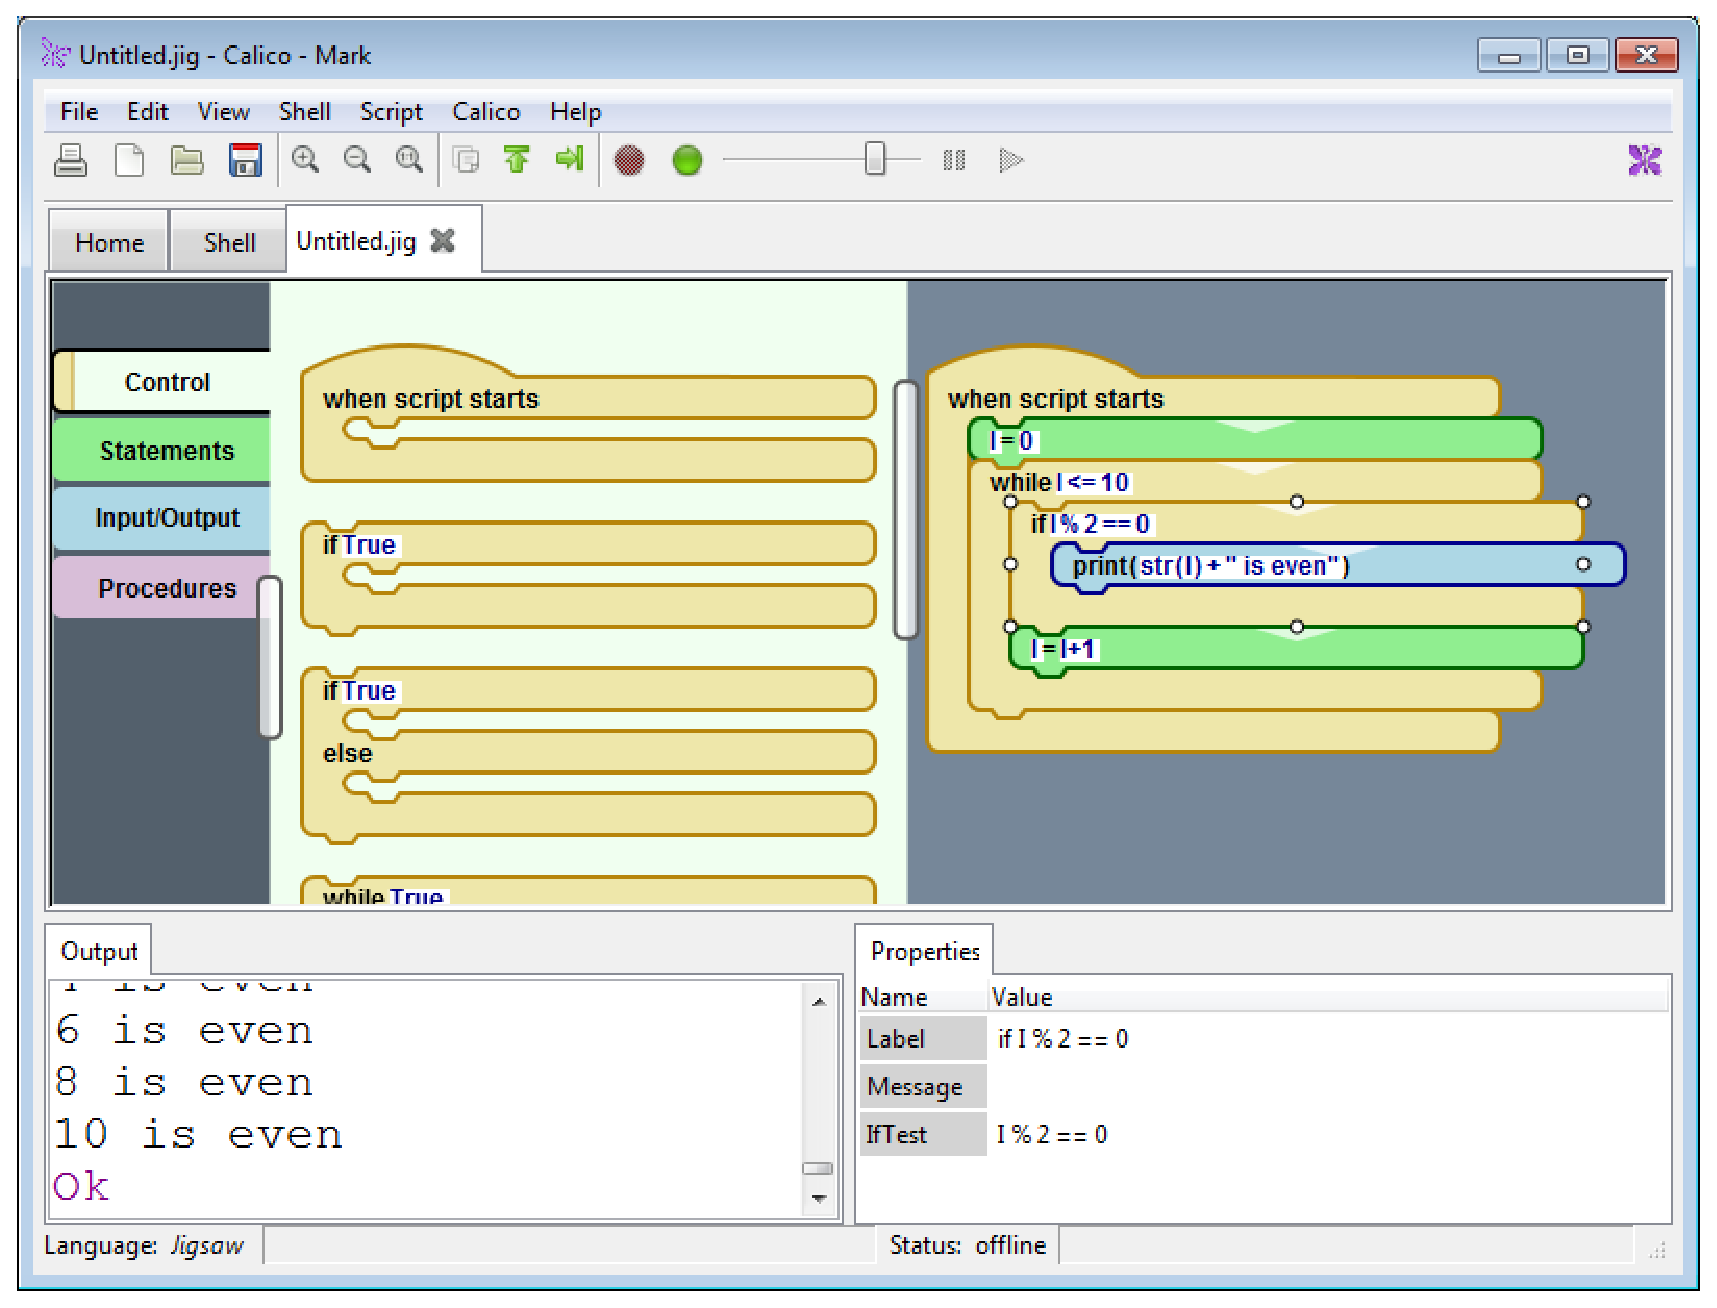
\includegraphics[width=75mm]{jigsaw2.eps} 
  \caption{Jigsaw blocks leverage Python expressions.}
  \label{jigsaw2}
\end{figure}

Although Jigsaw statements and expressions are borrowed from
Python, Jigsaw implements its own program control
structures. Blocks that provide looping, conditionals and procedures
are all implemented entirely in C\#. Program execution is managed
using Jigsaw's own implementation of call stacks and stack frames
along with local and global namespaces, an idea that is borrowed from
Python.

Another unique feature of Jigsaw is that it has a form of multitasking
baked in to its execution engine. A Jigsaw program begins execution at
a ``when script starts'' block, and proceeds down the attached stack
of blocks, executing each in sequence. But a Jigsaw program can
contain any number of ``when script starts'' blocks, which all begin
execution at the same time. As a result, a Jigsaw program can execute
multiple block stacks in parallel. See Figure~\ref{jigsaw3} for an
example. Blocks colored white indicate that it is currently being
executed.

\begin{figure}[h!]
  \centering
    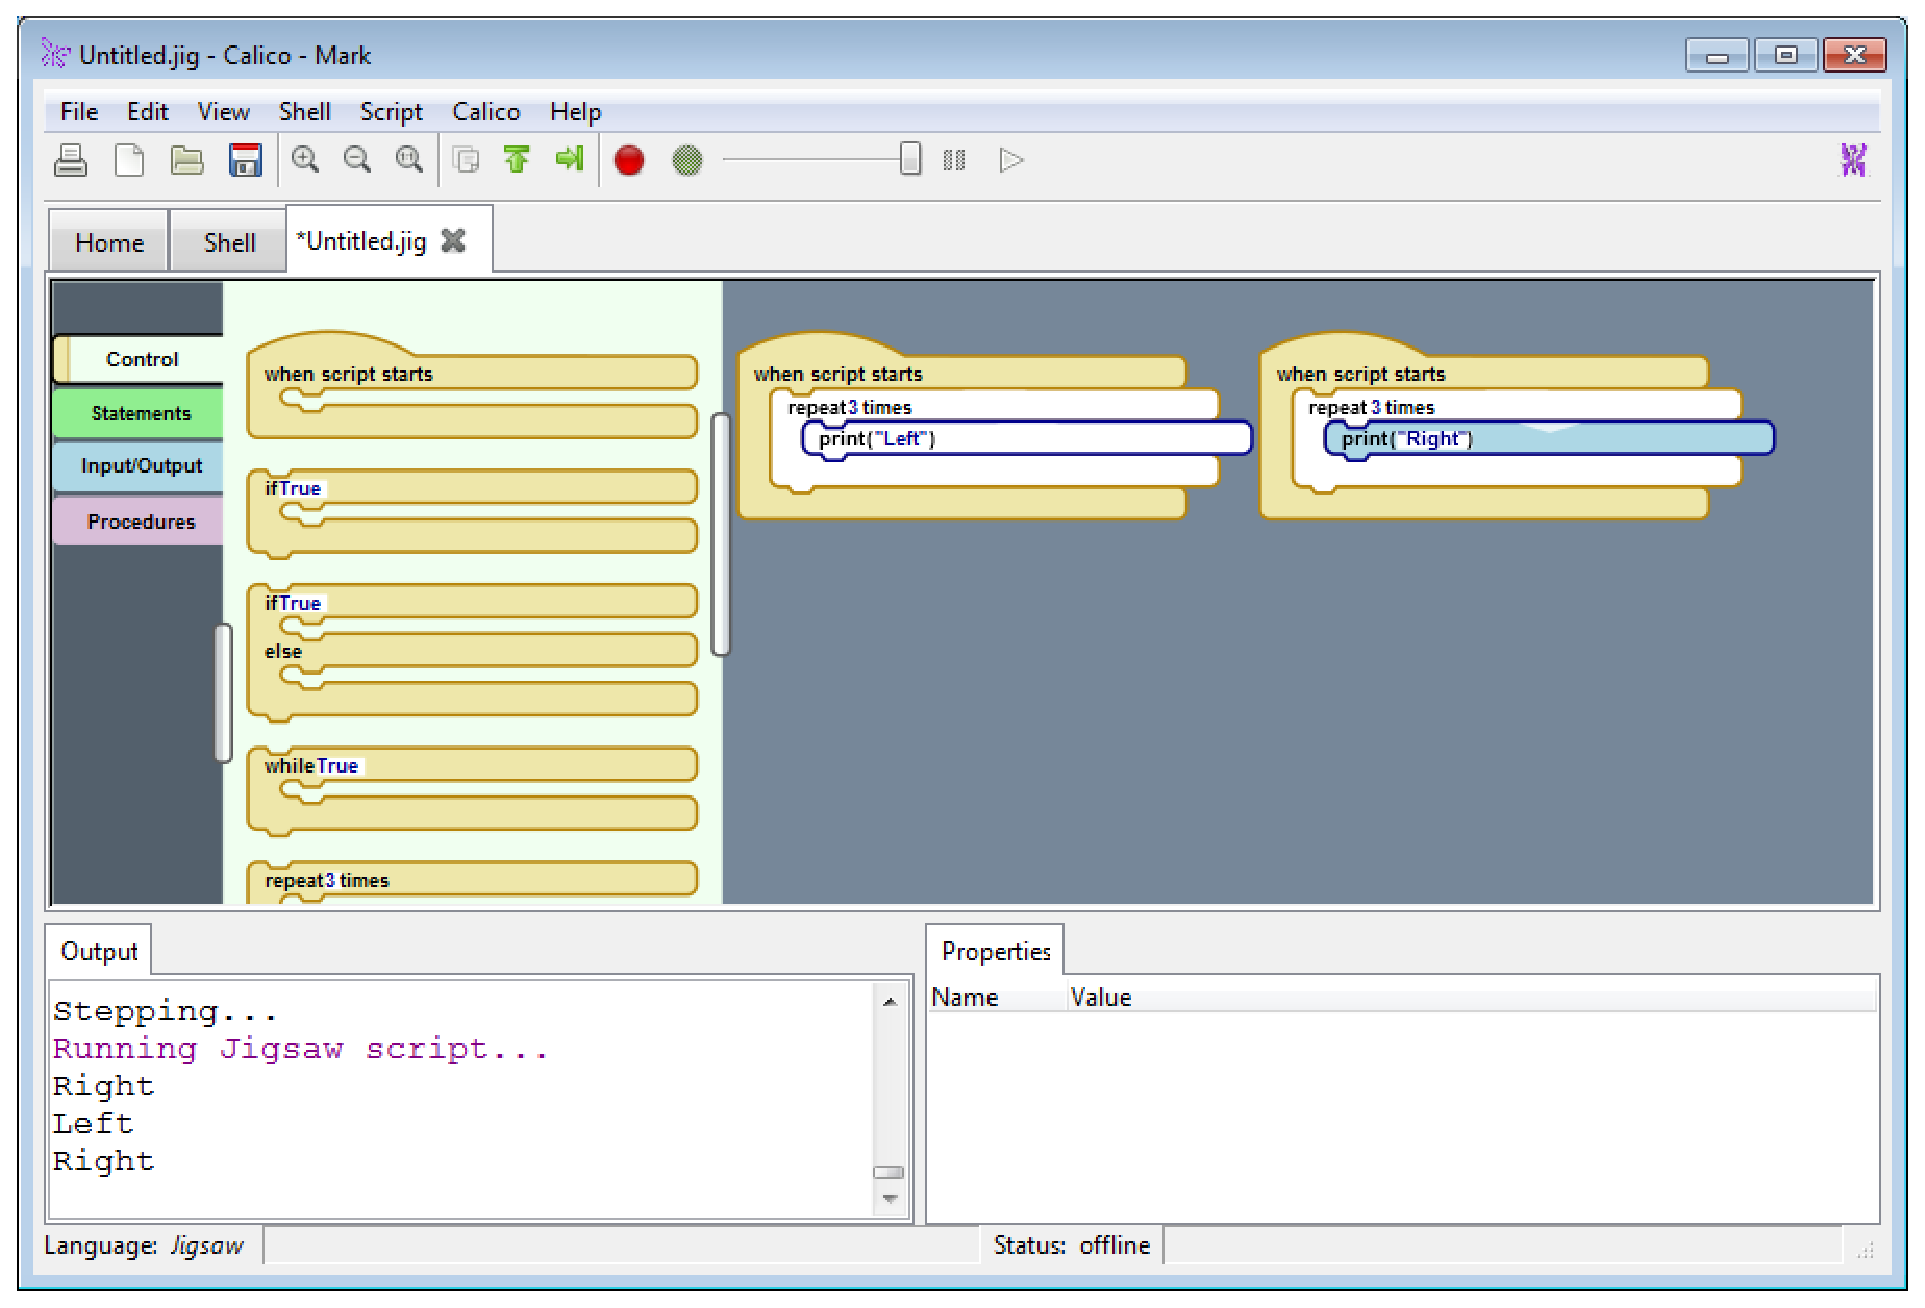
\includegraphics[width=75mm]{jigsaw3.eps} 
  \caption{A Jigsaw program running multiple block stacks in parallel.}
  \label{jigsaw3}
\end{figure}

The parallelism implemented in Jigsaw is a form of
cooperative multitasking, not the more common preemptive style. Jigsaw
executes multiple block stacks in a round-robin fashion. It is
important to note that the execution of one block does not necessarily
complete before the Jigsaw engine switches to a block in another
stack. Indeed, multiple blocks in different stacks can execute at the
same time. This is possible because block execution is implemented 
as a C\# Enumerator, which is carefully designed for each block type
to yield at safe places throughout its execution. With this
approach a novice programmer can assemble a program that
multitasks while avoiding the subtle bugs that often crop 
up with a true preemptive model. For example, a ``background'' task
that continuously monitors a sensor and updates a global variable 
can safely coexist with a second loop that uses the value of the global
variable to draw a graphic on the screen.

Calico Jigsaw allows the export of any Jigsaw script to Calico Python
(described below). However, to export it must convert Jigsaw's
controls to those of the Python language, the semantics must also be
converted. Figure~\ref{jigsaw4} shows the above Jigsaw program as it
appears after it has been exported to Python. Python does not have the
built-in ability to run functions simultaneously as does Jigsaw. But,
the Calico Myro module (described below) includes a friendly interface
for using threads through the ``doTogether'' function, and so the
export translates the Jigsaw program to the proper form. Notice,
however, that the Output tab indicates that Python's threads do not
guarantee even multitasking inside the for-block as the 'Left' and
'Right' outputs are not perfectly interleaved.

\begin{figure}[h!]
  \centering
    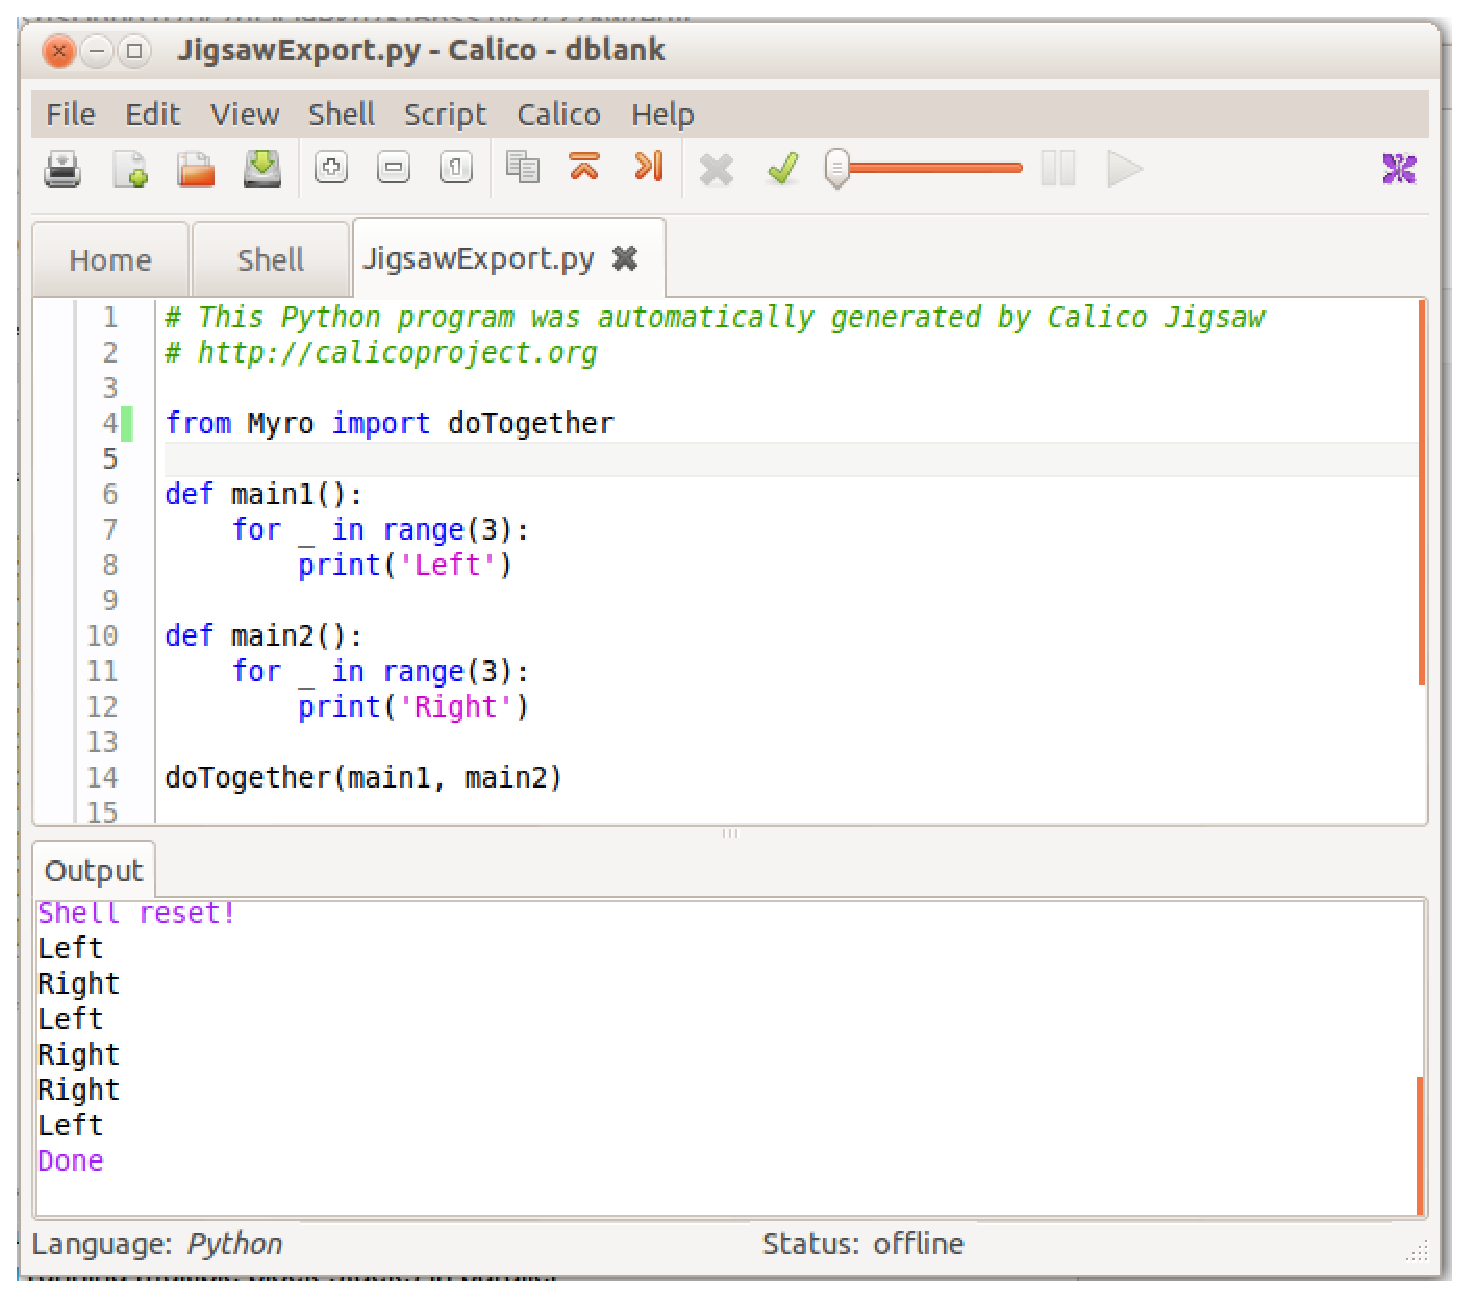
\includegraphics[width=75mm]{jigsaw4.eps} 
  \caption{The Jigsaw program from Figure~\ref{jigsaw3} exported
    as Python. Note that the blocks have been converted to functions
    (main1, and main2) but the output is not guaranteed to run in
    lockstep as it does with Jigsaw's multitasking.}
  \label{jigsaw4}
\end{figure}

\subsection{Calico Python and Ruby}

Calico Python is based on IronPython, with compiler options set to be
as much like Python 3 as possible. This includes treating print as a
function, and making the division operator produce a floating-point
number instead of the standard truncated integer, when a integer is
divided by another.

IronPython is the most developed and tested language using the DLR.
By default, a DLR-based language has the ability to use DLLs
directly. However, to make a language a first-class Calico language,
it must also provide debugger and interoperation
functionality. Because of the DLR, this additional functionality was
fairly easy to implement.

Likewise, Calico Ruby is based on IronRuby. Although not as well
developed, IronRuby is a very complete implementation of the
language. Calico Ruby is currently a second-class language, as we have
not implemented the stepping support needed.

\subsection{Calico Scheme}

We wrote a properly tail-recursive implementation of Scheme from
scratch and integrated it into Calico.  Tail-recursion is an idiom
that students often discover on their own as a way of implementing
iteration \cite{blank-kumar-2010}. Unfortunately, most of the
languages commonly used in introductory courses (for example, Java,
Python, and C++) do not handle tail-recursion correctly, which may
lead to crashes if a student's program exceeds the language's
recursion depth limit. This is seen by students as a bug in their
code, whereas it is really a limitation of the underlying language
implementation. Unlike other Scheme implementations for the MVM,
Calico Scheme does not rely on the underlying call stack of the
implementation language to manage function calls, nor does it require
functions to be compiled to Common Language Runtime (CLR)
bytecode. Consequently, tail calls are handled properly in Calico
Scheme, as required by the Scheme language specification
\cite{sperber-etal-2010}, imposing no limit on the depth of the call
stack (aside from system memory limitations).

Our Scheme implementation is itself written in Scheme, utilizing full
continuation-passing style (CPS).  Because the interpreter is in CPS, adding
support for new types of control structures or other language constructs to
Calico Scheme is easy.  We wrote a transformation program to automatically
transform the high-level CPS code into a low-level trampolined register machine
\cite{EOPL3}.  Although the resulting register machine code is still in Scheme,
it does not rely on Scheme's call stack, higher-order procedures, or
parameter-passing mechanisms.  Thus it can be translated directly into
low-level C\# code and then compiled for the MVM.
 
Calico Scheme supports all of the main language features of standard Scheme,
such as first-class procedures and continuations, but also adds several new
features of it own.  For example, we included support for exception handling in
the form of \texttt{try}, \texttt{catch}, \texttt{finally}, and \texttt{raise}
expressions.  Of course, the equivalent functionality can also be easily
achieved with \texttt{call/cc}, but since many students may already be familiar
with exception handling constructs in Java or Python, we decided to include
similar types of constructs in Calico Scheme as well.  To aid in debugging when
an exception is thrown, we implemented a user-configurable stack-trace
reporting mechanism that mimics the appearance of stack traces generated in
Python.  We also included support for McCarthy's nondeterministic choice
operator \texttt{amb} \cite{AMB}, called \texttt{choose} in Calico Scheme.
This allows students to easily explore the very different---and very
powerful---paradigm of nondeterministic computing, to which most of them have
probably not been exposed before.

The current transformation of Calico Scheme into C\# does not use the
AST from the DLR. Therefore, our current version runs quite a bit
slower than it could. However, to move to the DLR's AST, we will need
to define our own elements for handling continuations (see a
simple performance comparison, below). 

%Scheme has two forms of a stack-trace when an exception is thrown,
%depending on a user-set config. These are made to mimic those
%stack-traces of Python.

\subsection{Experimental Languages}

To add a language to Calico, one need only define a single function
that returns a Language class instance. In fact, Calico comes with a
fill-in-the-blank wizard for creating new text-based languages. For
text-based languages, one need only provide the language's name, a
string for beginning line comments, and the the language's source code
file extension (such as ``.py'' for the Python language). Further
details can help make the language more useful for programmers. Such
details include providing language keyword details for the IDE's color
syntax highlighting, and, of course, the language's parser and
interpreter. Because Calico supports calling other language, new
languages can be written in existing Calico languages. For example,
Calico's Basic and Logo languages are themselves written in Calico
Python. As another example, Calico Java's language definition is
written in Python, but the Java interpreter is written in Java
(described in more detail below).

One might want to use the Calico infrastructure for testing out a new
language. For example, if you had an interpreter (written in any
Calico language, or converted to use the MVM or JVM) then you could
put a light wrapper around it, and simply use the Calico IDE to make
it available. If you provide the keywords, and a few other items, you
could also have color syntax highlighting. If you add hooks to your
language to import Calico modules, then your experimental language
would have access to all of the included libraries (described
below). Finally, if you add a method to provide line numbers, and
intercept breakpoints, then your language would also be a first-class
Calico language.

Because it is so easy to add a new language to Calico (given that such
a language might initially be a second-class language with little
connection to the rest of Calico) there are a few languages that have
been initiated, but which have limited integration in Calico.

\subsubsection{Calico Java}

Calico Java is an example of a second-class language in the
ecosystem. However, the technology to bring it into the Calico fold is
quite interesting. We use the Java interpreter from DrJava
\cite{drjava}. Unfortunately that code is written in Java. Using IKVM,
we convert the Java bytecode directly to MVM bytecode. Thus, Calico can parse
and interpret Java in the MVM.

Even more interesting, to allow Calcio Java to use the Calico DLL modules,
they needed to be able to be consumed from the Java side. So, the DLL
modules were converted to jar files via IKVM. Therefore, the Calico
modules can be used in the Java, both the real JVM and also our Java
interpreted.

The complete effect is that Calico Java can load jar files that were
once DLLs, but interprete the language in the MVM rather than the
JVM. Unfortunately, the DrJava interpreter needs additional support
for stepping, access to line number when errors are encountered, and
access to other languages to be able to make Java a first-class Calico
language.

\subsubsection{Calico Basic, Logo}

Because all of the languages live in the same environment, it is easy
to develop a new Calico language in one of the existing Calico
languages. For example, Calico Basic and Calico Logo are both
interpreters written in Python. We have added the ability of both of
those languages to use Calico libraries; however, neither has
debugging support. Thus, both Logo and Basic are now languages with
access to all of the Calico libraries. For example, one can write
programs in these languages with access to the modern libraries, such
as Processing, Arduino, and robots (described below).

\subsection{Performance}

Compared to other dynamic languages, the performances of Calico
languages ranges from competitive to slow
\cite{python-benchmark}. Likewise, between Calico languages, there is
also large performance variability. Some of these differences can be
mitigated over time with refinements at various levels of
implementations. For example, Calico Scheme has yet to be converted to
use the DLR AST. Once that transformation is in place, we expect a 10
to 100-fold increase in performance. Other differences are likely to
remain, however. For example, Calico Basic is written in Calico
Python, so speed improvements will probably be minimal.

\begin{table}[h!]\footnotesize
  \centering
  \begin{tabular}{ l | l }
    \hline                        
    \textbf{Language} & \textbf{Time (in Seconds), Factorial of 1000} \\
    \hline                        
    Calico Scheme (non-recursive) & 0.002 \\
    CPython (recursive)           & 0.003 \\
    Calico Python (recursive)     & 0.020 \\
    Calico Ruby (recursive)       & 0.024 \\
    Calico Basic (using goto)     & 0.053 \\
    Calico Jigsaw (recursive)     & 0.072 \\
    Calico Scheme (recursive)     & 0.368 \\
  \end{tabular}
  \caption{Performance comparison between languages on a simple
    function: computing the factorial of 1000.}
  \label{performance}
\end{table}

\subsection{Interoperations}

As mentioned, first-class languages can call functions and use values
directly from other languages. There are two methods for running code
in one language from another: \textit{Evaluate} and
\textit{Execute}. Both of these methods are contained in the
\texttt{calico} global environment variable. Like their names suggest,
\texttt{calico.Evaluate} will evaluate an expression in the given
language, and return the result, while \texttt{calico.Execute} will
execute a series of statements in the given language for their
side-effects.

One reason one might do this is to convert from a type in one language
to a type in another. As a simple example, if you were writing Scheme
code, but wanted to create a Python tuple, then you could define, and
call, a Scheme function to take any number of arguments and return a
Python tuple (see Figure~\ref{scheme1}).

\begin{lstlisting}[language=Lisp, morekeywords={define}, caption={Defining a function \texttt{pytuple} in 
      Calico Scheme that directly uses Calico Python's lambda to construct a Python tuple. Notice     
      that in line 7 that the tuple's displayed representation reflects the style
      from Python rather than Scheme's.}, label={scheme1}]
scheme> (define pytuple 
          (calico.Evaluate 
             "lambda *args: args" 
             "python"))
Ok
scheme> (pytuple 1 2 3)
(1, 2, 3)
Ok
\end{lstlisting}

A more interesting example is calling a Scheme function from
Python. One might wish to do this, for example, because of Scheme's
lack of limitations on a recursive stack size. To call a Scheme
function requires that we connect Scheme's function-calling machinery
to the standard MVM function-calling system. This is a three step
process:

\begin{enumerate}
\item Write a regular (perhaps recursive) Scheme function 
\item Place the Scheme function in a MVM-compatible function wrapper
\item Make the wrapper available in the shared global environment
\end{enumerate}

For example, consider defining a recursive function to compute if a
number is even. In Python, there is a limited function-calling stack
size (set differently depending on the version of Python), whereas
Scheme has no such limitation as mentioned. In
Listing~\ref{callingscheme} we first define the iseven? function
(lines 1 -- 7). Line 9 does two things: it wraps the iseven? function
in a MVM function-calling wrapper using the Scheme primitive
\texttt{func}, and also places the new function in the global
environment, using the Scheme primitive \texttt{define!}. At this
point, any Calico language with access to the global environment can
now call the \texttt{iseven} function without worrying about recursion
depth.

\begin{lstlisting}[language=Lisp, keywords={define, lambda, cond, else, func, define!}, caption={Calling Scheme from Python.}, label={callingscheme}]
scheme> (define iseven?
         (lambda (n)
            (cond
                ((= n 0) #t)
                ((= n 1) #f)
                ((< n 0) (iseven? (- n)))
                (else (iseven? (- n 2))))))
Ok
scheme> (define! iseven (func iseven?))
Ok
\end{lstlisting}

If one of the languages is not a first class Calico language, they can
still interoperate. For example, as mentioned, Java is not currently a
first-class Calico language, but you can still execute statements, and
evaluate expressions from any language that has access to the calico
object. In the example in Listing~\ref{callingjava1}, Calico Python
calls Java to create a variable with a particular value.

\begin{lstlisting}[language=Python, caption={Calling Java from Python.}, label={callingjava1}]
python> calico.Execute("int x = 1;", "java")
Ok
python> pyx = calico.Evaluate("x", "java")
Ok
python> print(pyx) 
<java.lang.Integer object at 0x002B [1]>
Ok
python> print(pyx.intValue())
1
Ok
\end{lstlisting}

The value of \texttt{pyx} is actually a value directly from the Java
world: a \texttt{java.lang.Integer} object. To convert it to a MVM value
depends on the specifics of the foreign system. In this case,
calling \texttt{pyx.intValue()} is required.

\subsection{Current Limitations and Future Work}

As Calico is a work-in-progress, there are many directions to
explore. For example, Calico cannot currently directly use C-based
libraries.  However, this limitation could be overcome (see the
IronClad project for IronPython \cite{ironclad}). Currently, there are
a limited number of exports from one language to another. We believe
that having additional exports between languages would facilitate
learning transfer and transitions from one language to another.
Finally, we are working to move more languages from their second-class
status to be full first-class languages.

%% In addition, Kolling mentioned in his keynote address at SIGCSE this
%% year that he believes that we may be ready for a "structural editors"
%% rebirth. And this would be for experts. Paraphrasing, his idea is to
%% blend text editing with the idea of blocks (or "structures"). We can
%% tip our hat to the idea that "blocks" can be productive to experts
%% too.

\section{Calico Modules}

A Calico ``module'' is a library written in such a manner that it is
available to all of the Calico first-class languages. However, not
only is the functionality in the module available to these languages,
but the modules appear as if the are a native library to each
language. For example, in Calico Python one would write ``import
Processing'' to make the Calico Processing module (discussed below)
available to Python. One could then write ``Processing.window(400,
300)'' in Python to create a 400x300 pixel window. In Scheme, one
would write ``(using "Processing")'' to make the Calico Processing
module available to Scheme. One could then write ``(Processing.window
400 300)'' in Scheme to do the same thing. Finally, in Calico Jigsaw,
selecting ``Use a Module; Processing'' from the menu would allow the
window-block to be dragged onto the Jigsaw workspace. Thus, the
Processing module is written and compiled once, becomes available to
all of the first-class Calico languages, and used as if it were
written as a native language. Likewise, if a new first-class language
is introduced into the Calico ecosystem, all of these modules can be
used by the new language.

To create a Calico module, a single file is written and compiled once
to a Dynamic Link Library (DLL). There are DLL files that are
Windows-specific; however, these DLLs are platform-neutral and can be
created on any operating system for use on any other operating
system. To remain platform-neutral these DLL's must be written such
that they do not take advantage of Windows-specific functionality, do
not rely on lower-level platform-specific C libraries (e.g., are
completely ``managed''), and use a subset of all possible
functionality. Currently, to be accessible to all Calico languages, we
currently restrict the module to only use static class methods in a
toplevel-defined class. However, this limit could be relaxed in a
future Calcio to allow more flexibility (constructors, nested classes,
etc). In general, any managed DLL could be fully utilized by a
properly flexible, dynamic, first-class languages, but might require
specific knowledge about the layout of the internal classes, methods,
and namespaces. Thus, we have specified a subset of all that is
possible for our own modules so that no additional knowledge or
discovery is needed.

\begin{lstlisting}[language=Java, caption={Example module template.}, label={csharp-module}]
// C# ModuleName.cs compiles to ModuleName.dll
public class ModuleName {
    public static int Plus(int a, int b) {
        return (a + b);
    }
}
\end{lstlisting}

If the code in Figure was compiled and placed into the Calico/modules
folder, then it could be used in Python (as in the form \texttt{import
ModuleName}, Scheme (as in the form \texttt{(use "ModuleName")} and in
Jigsaw and all of the other Calico languages, in their respective
forms. We now explore three modules that provided a variety of
functionality for Calico first-class languages.

\subsection{Processing}

Calico Processing is a module for developing digital works of art,
data visualizations, interactive applications and animations. It
offers Calico programmers the option to work with the familiar and
popular \textit{Processing} command set (see \cite{processing}). The Calico
Processing module attempts to be faithful to the Processing command
set, including function names, arguments, and usage. The majority of
the command set has been implemented, although some differences exist.

The original Processing language is a subset of Java with a wide variety of
commands included for creating visualization and animations. The
Calico Processing module brings the Processing command set to all of the Calico
programming languages that can access Calico modules. This module does not make use of the Java
language syntax. Instead, native data types and control structures of
your chosen Calico language will determine how your application is
constructed.

We rely upon each of the native Calico languages for the following capabilities:

\begin{itemize}
\item Data structures
\item Program control (conditionals, iterations, etc.)
\item Files and file access
\item String functions
\item Objects and inheritance
\end{itemize}

Mouse and keyboard events are not handled by implementing predefined
functions. The Calico Processing module raises events, which are
handled by the native language event handling syntax. Events raised by
the module include onMousePressed, onMouseReleased, onMouseClicked,
onKeyPressed, and onKeyReleased. Loops are implemented by handling a
timer tick event named onLoop.

Certain predefined fields in Processing are implemented as functions.

\begin{itemize}
\item ''mouseX'' and ''mouseY'' are implemented in Calico Processing as the functions ''mouseX()'' and ''mouseY()''.
\item ''pmouseX'' and ''pmouseY'' are implemented as ''pmouseX()'' and ''pmouseY()''.
\item ''width'' and ''height'' are implemented as ''width()'' and ''height()''.
\item ''focused'' and ''frameCount'' are implemented as ''focused()'' and ''frameCount()''.
\item ''key'' and ''keyCode'' are implemented as ''key()'' and ''keyCode()''.
\end{itemize}

The result is a pixel-by-pixel faithful representation of the original
Processing primitives' output. However, combined with the Calico
dynamic languages, the Processing module provides functionality not
available within the original Processing environment. For example,
Calico allows the drag-and-drop creation of Processing art via Jigsaw,
line-by-line stepping through programs, and breakpoints by using any
of the Calico first-class languages.

The Calico Processing module is similar in some respects to the port
of the original Processing commands to the Python library
\textit{pyprocessing} \cite{pyprocessing}, and perhaps other ports to
specific languages. However, our module has been written, and
compiled, just once and is then available to all of the Calico
languages. In addition, the pyprocessing has additional dependencies
that must be maintained and installed.

\subsection{Myro and Graphics}

Calico comes with a rich library for exploring robots, called
Myro. The Myro module allows students to control a real or simulated
robot, take pictures, do image processing, make the robot speak, go
through a maze, draw a picture, etc. The Myro library is described in
detail in \cite{blank-etal-2012}.

The Calico Graphics module is a 2D graphics library for creating art,
games, and animations in any of the Calico languages. The Calico
Graphics module forms the basis for the Physics-based simulations and
animations (for use in creating games such as Angry Birds) and
contains GIS functionality. A full reference of the Calico Graphics
module can be found at \cite{calico-graphics}.

\section{Conclusion}

The Calico project was designed to be a dynamic languages ecosystem
for learning, exploring, creating, and using dynamic languages, both
individually, and in cooperation with each other. It defines a
multi-language, multi-context programming framework and learning
environment for computing education and research. The ecosystem is
designed to support several interoperable programming languages
(including Python, Scheme, and Jigsaw) running on a universal virtual
computer, a variety of pedagogical modules (including robotics, and
art), and an assortment of physical devices (including different
educational robotics platforms and a variety of physical sensors). In
summary, we hope that Calico will provide a long-term, robust
ecosystem that can be used to create and sustain a community of
researchers, educators, and students working together.

%%\appendix
%%\section{Appendix Title}

%%This is the text of the appendix, if you need one.

\acks

The Calico Project grew out of research initially funded by Microsoft
Research under the Institute for Personal Robots in Education, and
then the National Science Foundation, grant DUE-0920539. In addition,
we would like to thank the many students, teachers, and other
explorers who have provided invaluable feedback on Calico.

% We recommend abbrvnat bibliography style.

\bibliographystyle{abbrvnat}

% The bibliography should be embedded for final submission.

\begin{thebibliography}{}
\softraggedright

\bibitem[]{java-davinci}
%% Details on Da Vinci Machine for the JVM
Da Vinci Machine for the JVM.\\ URL http://openjdk.java.net/projects/mlvm/pdf/LangNet20080128.pdf Accessed June 6, 2013.

\bibitem{java-lambda}
Project Lambda for the JVM.\\ URL http://openjdk.java.net/projects/lambda/ Accessed June 6, 2013.

\bibitem{java-jigsaw}
Project Jigsaw for the JVM.\\ URL http://openjdk.java.net/projects/jigsaw/ Accessed June 6, 2013.

\bibitem{java-nashorn}
Project Nashorn for the JVM.\\ URL http://openjdk.java.net/projects/nashorn/ Accessed June 6, 2013.

\bibitem{ironpython}
IronPython.\\ URL http://ironpython.codeplex.com/ Accessed on January 12, 2012.

\bibitem{ironruby}
IronRuby.\\ URL http://en.wikipedia.org/wiki/IronRuby Accessed on June 6, 2013.

\bibitem{gtk-sharp}
GtkSharp.\\ URL http://www.mono-project.com/GtkSharp Accessed on January 12, 2012.

\bibitem{sdl}
Simple Direct Media Layer.\\ URL http://www.libsdl.org/ Accessed on June 6, 2013.

\bibitem{csharp-sdl}
C\# SDL, wrapper for SDL.\\ URL http://cs-sdl.sourceforge.net/ Accessed June 6, 2013.

\bibitem{pygame}
Pete Shinners. Python Pygame Introduction.\\ URL http://www.pygame.org/docs/tut/intro/intro.html Accessed on June 6, 2013.

\bibitem{ikvm}
IKVM Homepage.\\ URL http://www.ikvm.net/ Accessed June 6, 2013.

\bibitem{wu-2010}
Chaur Wu. 2010. \textit{Pro DLR for .NET 4}. Apress, 2010.

\bibitem{calico-project}
Calico Project.\\ URL http://calicoproject.org/ Accessed June 6, 2013.

\bibitem{blank-etal-2012} Douglas Blank, Jennifer S. Kay, James
  B. Marshall, Keith O'Hara, and Mark Russo. \textit{Calico: A
    Multi-Programming-Language, Multi-Context Framework Designed for
    Computer Science Education}.  SIGCSE’12, February 29–March 3,
  2012, Raleigh, North Carolina, USA.

\bibitem{blank-ohara-2013} Douglas Blank and Keith
  O'Hara. \textit{The Calico Project for Robots in
    Education}. 2013. Under review.

\bibitem{jrose12}
%% Details on upcoming dynamic language support for Java
J. Rose. Lang Next.\\ URL
http://cr.openjdk.java.net/~jrose/pres/201204-LangNext.pdf Accessed
June 6, 2013.

\bibitem{squeakvm}
%% Lists many via VMs, including Squeak
Squeak Virtual Machine.\\ URL http://www.squeak.org/Features/TheSqueakVM/ Accessed June 6, 2013.

\bibitem{vm-compare} Comparison of application virtual machines.\\ URL
  http://en.wikipedia.org/wiki/Comparison \_of\_application\_virtual\_machines
  Accessed June 6, 2013.

\bibitem{python-benchmark} IronPython Performance. \\ URL
  https://ironpython.codeplex.com/wikipage?title=IP27A1VsCPy27Perf
  \&referringTitle=IronPython\%20Performance Accessed June 6, 2013.

\bibitem{ecma-standards} Ecma Standards.\\
URL http://www.mono-project.com/ECMA Accessed on January 12, 2012.

\bibitem{mono} Mono Virtual Machine and Runtime.\\ URL http://en.wikipedia.org/wiki/Mono\_(software) Accessed June 6, 2013.

\bibitem{microsoft-community-promise} Microsoft Community Promise. 2007.\\
URL http://www.microsoft.com/interop/cp/ Accessed June 6, 2013.

\bibitem{espeak} eSpeak, text-to-speech.\\ URL http://espeak.sourceforge.net/ Accessed June 6, 2013.

\bibitem{steinart-etal-2012} Bastian Steinert, Damien Cassou, and
  Robert Hirschfeld. \textit{CoExist: Overcoming Aversion to
    Change}. DSL'12.

\bibitem{dlr-wikipedia} Dynamic Language Runtime.\\ URL
  http://en.wikipedia.org/wiki/Dynamic\_Language\_Runtime Accessed
  June 6, 2013.

\bibitem{blank-kumar-2010} Douglas Blank and Deepak
  Kumar. 2010. \textit{Assessing the Impact of using Robots in
    Education, or: How We Learned to Stop Worrying and Love the
    Chaos}. 2010. AAAI Spring Symposium Series, Educational Robotics
  and Beyond: Design and Evaluation, Palo Alto, California, March 22,
  2010 – March 24, 2010.

\bibitem{ipre-2008} Tucker Balch, Jay Summet, Douglas Blank, Deepak Kumar,
  Mark Guzdial, Keith O'Hara, Dan Walker, Monica Sweat, Gaurav Gupta,
  Stewart Tansley, Jared Jackson, Mansi Gupta, Marwa Muhammad, Shikha
  Prashad, Natasha Eilbert, Ashley Gavin. 2008. \textit{Designing
    Personal Robots for Education: Hardware, Software, and
    Curriculum}. Pervasive Computing, IEEE, volume 7, Issue 2, pages 5
  - 9. April 2008.

\bibitem{blank-2006} Douglas Blank. 2006. \textit{Robots make computer science
  personal}. Communications of the ACM 49, 12, 25-27.

\bibitem{powershell} PowerShell. URL http://en.wikipedia.org/wiki/PowerShell Accessed June 6, 2013.

\bibitem{sperber-etal-2010} Michael Sperber, R. Kent Dybvig, Matthew
  Flatt, Anton van Straaten, Robby Findler, Jacob Matthews
  (editors). 2010. \textit{Revised [6] Report on the Algorithmic Language
  Scheme}. Cambridge University Press. April 2010.

\bibitem{AMB} J. McCarthy, 1963. ``A Basis for a Mathematical Theory
  of Computation'', in P. Braffort and D. Hirshberg (Eds.),
  \emph{Computer Programming and Formal Systems}, North-Holland.

\bibitem{EOPL3} D. Friedman and M. Wand, 2008. \emph{Essentials of
  Programming Languages, 3rd edition}. MIT Press.

\bibitem{scratch} John Maloney, Mitchel Resnick, Natalie Rusk, Brian
  Silverman, and Evelyn Eastmond. 2010. \textit{The Scratch Programming
  Language and Environment}. Transactions on Computing Education 10, 4,
  Article 16 (November 2010).

\bibitem{dlr-microsoft} Dynamic Language Runtime Overview. \\ URL
  http://msdn.microsoft.com/en-us/library/dd233052.aspx Accessed June
  7, 2013.

\bibitem{drjava} Drjava. URL http://www.drjava.org/ Accessed June 8, 2013.

\bibitem{ironclad} IronClad. URL http://code.google.com/p/ironclad/
  Accessed June 8, 2013.

\bibitem{processing} Processing. URL http://processing.org/reference
  Accessed June 8, 2013.

\bibitem{pyprocessing}
  pyprocessing. http://code.google.com/p/pyprocessing/ Accessed June
  8, 2013.

\bibitem{calico-graphics} Calico Graphics Module. URL http://calicoproject.org/Calico\_Graphics Accessed June 8,
  2013.

\end{thebibliography}

\end{document}

